\section{Successor Representation} \label{sec: SR}
According to \etal{Stachenfeld}, our behavior in an open spatial environment, or in general in a \cognitiveroom{} \eg a city, follows the predictive map theory introduced in \secreff{sec: predictive map theory}. An active place cell encodes the next/successor state entered by the agent.

To model this or the general setting of predicting future states, the \gls{sr} was developed by a \gls{rl} approach. Furthermore, the \gls{sr} and the predictive map theory go hand in hand. The latter is an application regarding the former: The authors support the proposition that hippocampal mechanics, explained by the predictive map theory, can be described via the \gls{sr}.

% ======================================

\subsection{Mathematical Foundation}
The basis lies largely in \gls{rl}, in formula:
\begin{equation}\label{eq: rl}
	V(s) := E \left[
				\sum_{t=0}^{\infty}
					\gamma^t R(s_t) | s_0 = s
			\right]
\end{equation}
with $ V $ resembling a value function, expressed via the reward function $ R $, which operates on state $ s_t $, encoded by the sum over $ t $, starting in $ s $. $ \gamma \in [0,1] $ serves as a discount factor to control the influence of states reached in distant future. High values permit distal states to play a larger role, whereas smaller values de facto limit the result to neighboring positions\footnote{Short mathematical explanation: $ p^t \xrightarrow[]{t \to \infty} 0 $ for $ p \in [0,1) $, the greater $ p $ the slower happens the approach of the limit. For $ p = 1 $ the sequence is constant. In our case every state is taken into account equally.}. By the reward function is obtained how beneficial the currently visited state $ s_t $ is. % The expected value is taken because there are \wlog plenty of paths starting in $ s $.
After the calculation of $ V $, the function can be decomposed into a more intuitive representation, consisting of a state matrix $ M $, called the \srmat{}, and the known reward function $ R $:
\begin{equation}\label{eq: v with sr-matrix}
	V(s) = \sum_{s'}
				M(s, s') \cdot R(s')
	\text{.}
\end{equation}
The first argument of $ M $ specifies the row, the latter the column. Each cell contains the discounted expected number of times the agent visits state $ s' $ starting from $ s $. Additionally, \etal{Stachenfeld} mention that the \srmat{} can be derived from a transition probability matrix $ T $ for the positions $ s $~\cite{StBoGe17HPM}. Having $ T $, it follows
\begin{equation}\label{eq: sr or m via T}
	M = \sum_{t = 0}^{\infty}
			\gamma^t T^t
	\text{,}
\end{equation}
which is a geometric series and converges for $ \gamma < 1 $ towards
\begin{equation}\label{eq: geo series}
	(I_n - \gamma T)^{-1}
	\text{,}
\end{equation}
where $ I_n $ is the corresponding identity matrix.

Although defining all formulae by infinite sums, it is seamlessly possible to calculate the \srmat{} in \equref{\eqref{eq: sr or m via T}} up to a finite index or starting at an arbitrary $ t $ \ie $ t=1 $. Doing so makes sense in a language environment. The identity matrix would imply that a word can follow itself, which is extremely rare\footnote{Although sentences like ``Ich hoffe, dass das das Richtige ist.'' do occure in german.}. Therefore, the first summand will always be $ \gamma T $, where $ T $ is calculated by a Neural Network (\secreff{ch: framework}). If the indices in \equref{\eqref{eq: sr or m via T}} are altered, the limit of the geometric series no longer applies directly and has to be adjusted by subtracting the first summands from \equref{\eqref{eq: geo series}}. The \gls{sr} and thus the depicted formulas, especially the \srmat{} and the transition probability matrix, are policy dependent. This is reflected by the training data.

By definition, matrix $ M $ reveals all successor states with their particular probability because the summation combines the following positions, which are calculated by exponentiation, into one matrix. By examining a row (\figref{\ref{fig: sr-spalte}}) \eg row $ k $, it is possible to follow all paths starting from state $ k $.

One advantage of the \gls{sr}, \ie describing the model by the \srmat{} $ M $, is its high flexibility regarding the evaluation of different reward functions given by \equref{\eqref{eq: v with sr-matrix}}. The value of a state $ s $ can be calculated in an instant with a different reward function while no relearning is necessary.

\paragraph{\gls{sr} and grid cells}
Although not further discussed in the thesis but an interesting claim of \etal{Stachenfeld} is that the eigenvalue decomposition of the \srmat{} reveals the grid cell structure. They provide supplementary information depicting many examples~\cite{StBoGe17HPM}.

% ======================================

\subsection{Example for the Successor Representation}
This subsection is dedicated to fill the concept of the \gls{sr} and the \srmat{} $ M $ with some intuition. \etal{Stachenfeld} simulated a linear spatial environment built by six states with a simple policy merely consisting of two actions the agent can apply: Going one step to the right or pausing.
%
\paragraph{Rows}
In this scenario, a plot of single rows of $ M $ is shown in \figref{\ref{fig: sr-zeile}}.
\begin{figure}
	\centering
		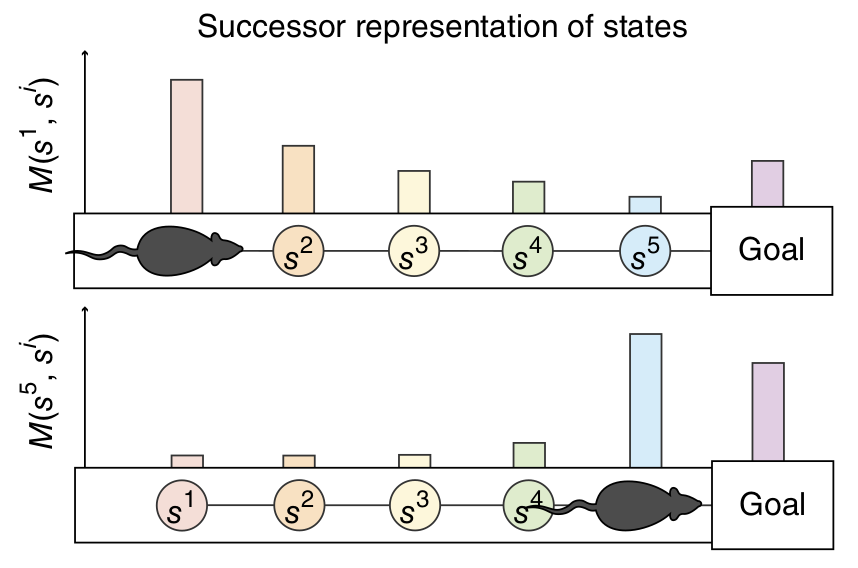
\includegraphics[width=0.7\linewidth]{Beispiel_SR_Zeile.png}
	\caption{Schematic plot of the rows of state $ s^1 $ and $ s^5 $ respectively. By interpreting the ordinate values as probabilities for transitioning instead of a probability for the current state, it is possible to make assumptions on the future path the agent may take. Hence, matrix $ M $ describes all possible paths. In both cases the policy prefers pausing over changing the state.}
	\label{fig: sr-zeile}
\end{figure}
From the upper half of \figref{\ref{fig: sr-zeile}}, examining the row of $ s^1 $, it is possible to deduce that the agent will most likely remain at its current position, with the values for distal locations disappearing. A different point of view results for the part of $ M(s^5, s^i) $. It is obvious that going backwards is nothing to reckon with since the numbers for transitioning distribute over $ s^5 $ and \texttt{goal} by slightly favoring the former. This behavior was expected by the policy.
%
\paragraph{Columns}
It is also worth analyzing the columns of $ M $, called \emph{place fields} by \etal{Stachenfeld} (\figref{\ref{fig: sr-spalte}}). Having the policy in mind, it is no surprise that the values $ M(s^i, s^5) $ ascend in parallel to the index $ i $. The probability for entering $ s^5 $ grows by approaching it. In addition the plot shows how $ s^5 $ is probably reached best, simply by passing via $ s^3 $ and $ s^4 $. This might seem obvious, but in a more complex \cognitiveroom{} the graph won't look as ordinary and therefore will contain plenty of distributed information. %A spike on $ s^1 $ would counteract it because it means stepping from $ s^1 $ to $ s^5 $ directly (as seen in Fig. \ref{fig: sr-zeile} this is not the case).
\begin{figure}
	\centering
		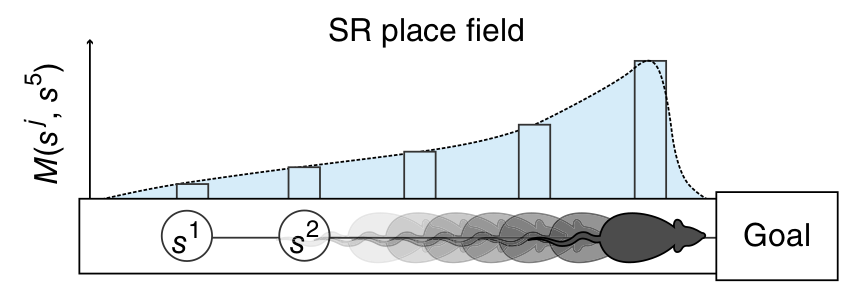
\includegraphics[width=0.7\textwidth]{Beispiel_SR_Spalte.png}
	\caption{Schematic plot of the $ s^5 $-column depicting how $ s^5 $ is reached by ascending probabilities. It is possible to recapitulate the policy consisting of pausing or taking one step to the right. Entering $ s^5 $ is most likely from $ s^4 $ and $ s^5 $ (due to resting). }
	\label{fig: sr-spalte}
\end{figure}
